\documentclass[11pt,a4paper]{article}
\usepackage[margin=1in]{geometry}
\usepackage[T1]{fontenc}
\usepackage[utf8]{inputenc}
\usepackage{amsmath,amssymb,amsfonts}
\usepackage{graphicx,booktabs,float,caption,xcolor,listings}
\usepackage[hidelinks]{hyperref}
\usepackage{microtype}
\captionsetup{font=small}
\setcounter{tocdepth}{1}
\lstset{language=Python,basicstyle=\ttfamily\scriptsize,keywordstyle=\color{blue!70!black},
commentstyle=\color{green!40!black},stringstyle=\color{red!60!black},
numbers=left,numberstyle=\tiny\color{gray},numbersep=6pt,showstringspaces=false,
breaklines=true,frame=single,rulecolor=\color{black!40},tabsize=4}
\newcommand{\GBMEMRate}{0.500}
\newcommand{\GBMEMWeakRate}{0.999}
\newcommand{\GBMMilRate}{0.991}
\newcommand{\GBMMilWeakRate}{1.000}
\newcommand{\GBMAnalyticWeakRate}{0.9993}
\newcommand{\GBMFitWindow}{$N=64,128,256,512,1024$}
\newcommand{\GBMExactMean}{105.1987}
\newcommand{\GBMExactVariance}{1045.0120}
\newcommand{\GBMExactMeanCI}{[105.0403, 105.3571]}
\newcommand{\NARate}{0.491}
\newcommand{\NAFitWindow}{$N=8,16,32,64$}
\newcommand{\NAExactMean}{105.08796}
\newcommand{\NAExactMeanCI}{[104.89962, 105.27629]}
\newcommand{\NAPayoff}{14.53804}
\newcommand{\NAPayoffCI}{[14.40515, 14.67093]}
\newcommand{\NAWeakInterpretation}{The 95\% intervals include zero at $N=64,128,256$. No weak order is assigned to the complete grid range. The finest-reference payoff is estimated as 14.53804 with interval [14.40515, 14.67093].}
\newcommand{\NAReferenceInterpretation}{The last refinement discrepancy is 0.04016. It is 3.2\% to 8.9\% of the coarse strong differences on the prespecified fitting window. This meets the practical 10\% reference-sensitivity criterion used for that window. For $N=256$, the ratio is 18.0\%, so the finest coarse points are retained as sensitivity evidence, not used for the principal rate claim. The two refinements decrease the strong discrepancy; their paired payoff intervals assess whether the benchmark changes at a detectable weak scale. Neither a small refinement difference nor a zero-containing interval is a rigorous bound on the unknown continuous-time error.}

\title{Numerical Simulation of Financial SDEs\\
\large Problem 4 GBM Benchmark and Non-Affine Volatility}
\author{Coursework Report}
\date{September 2026}
\begin{document}
\maketitle
\begin{abstract}
This report compares exact simulation, Euler--Maruyama (EM), and Milstein for geometric Brownian motion (GBM), and then investigates a non-affine stochastic-volatility model for which a numerical reference is required. All discretisations are coupled through aggregated Brownian increments. For GBM, the measured terminal strong orders are \GBMEMRate{} for EM and \GBMMilRate{} for Milstein, consistent with orders $1/2$ and $1$. Weak mean bias is separated from Monte Carlo uncertainty using paired differences, independently fitted control variates, and an analytic discrete-mean identity. The terminal distribution is checked against the exact lognormal law. In the non-affine model, EM is applied to log price and the volatility factor, preserving positive prices. Its observed strong rate is \NARate{} on the stated fitting window. Payoff bias is reported with confidence intervals and three nested reference grids; unresolved biases are not assigned a convergence order. The experiments demonstrate why an exact benchmark validates a method, while agreement between numerical grids requires a separate reference-resolution assessment.
\end{abstract}
\tableofcontents
\vfill
\noindent\small Reproducibility: complete Python source, seeds, numerical tables, figures, and run logs accompany this report. Reported confidence intervals are pointwise Monte Carlo intervals.

\newpage
\section{Introduction and theoretical background}
The supplied problem pack selects an SDE pathway in which strong and weak convergence, sampling uncertainty, and nested-grid validation replace deterministic ODE stability-region and adaptive-step analyses \cite{pack}. This topic is useful because GBM offers an exact pathwise benchmark, whereas the prescribed non-affine model makes time discretisation part of the solution. The objective is to establish what the experiments actually validate, rather than infer accuracy from plausible-looking sample paths.

\subsection{GBM and its exact transition}
For $S_0>0$, the It\^o SDE and log transformation are
\begin{align}
dS_t&=\mu S_t\,dt+\sigma S_t\,dW_t,\\
dX_t&=(\mu-\tfrac12\sigma^2)\,dt+\sigma\,dW_t,\qquad X_t=\log S_t.
\end{align}
It\^o's correction is essential: omitting $-\sigma^2/2$ changes the mean.
Integration gives
\begin{equation}
S_t=S_0\exp\{(\mu-\tfrac12\sigma^2)t+\sigma W_t\}.
\label{eq:exact}
\end{equation}
Thus $S_T$ is lognormal, with
\begin{align}
m&=\mathbb E[S_T]=S_0e^{\mu T},\\
v&=\operatorname{Var}(S_T)=S_0^2e^{2\mu T}(e^{\sigma^2T}-1),\\
q_p&=S_0\exp\{(\mu-\tfrac12\sigma^2)T+\sigma\sqrt{T}\Phi^{-1}(p)\}.
\end{align}
For the chosen GBM baseline $S_0=100$, $\mu=0.05$, $\sigma=0.30$, $T=1$,
$m=105.1271$ and $v=1040.7868$ (rounded). GBM parameters are experiment choices; the non-affine parameters on page~\pageref{sec:protocol} are prescribed by the problem.

\subsection{Three methods on a common Brownian path}
Let $h=T/N$, $\Delta W_n\sim N(0,h)$. Exact simulation uses
\begin{equation}
S_{n+1}=S_n\exp\{(\mu-\tfrac12\sigma^2)h+\sigma\Delta W_n\}.
\end{equation}
The price-based EM and scalar Milstein updates are
\begin{align}
S_{n+1}^{E}&=S_n^{E}(1+\mu h+\sigma\Delta W_n),\label{eq:em}\\
S_{n+1}^{M}&=S_n^{M}\{1+\mu h+\sigma\Delta W_n+
\tfrac12\sigma^2[(\Delta W_n)^2-h]\}.\label{eq:mil}
\end{align}
The extra term follows from $\tfrac12 b(S)b'(S)[(\Delta W)^2-h]$ with $b(S)=\sigma S$ \cite{higham}. Under the usual regularity assumptions, terminal strong orders are $1/2$ and $1$; weak order is $1$ for suitable smooth test functions. Applying EM to the GBM log price instead is exact at grid points. Its additive-noise Milstein correction vanishes, so it cannot demonstrate a nontrivial order-one comparison.

\newpage
\section{Monte Carlo methodology}
\subsection{Coupling and uncertainty}
Generate independent paths on the finest grid. A coarse Brownian increment is the sum of the corresponding fine increments, so
\begin{equation}
\Delta W_n^{(h)}=\sum_{j=nr}^{(n+1)r-1}\Delta W_j^{(\delta)},
\qquad h=r\delta.
\label{eq:coupling}
\end{equation}
For GBM, the exact terminal value uses the same total $W_T$.
For non-affine volatility, coarse and reference states use the same paired Brownian drivers. Independent random numbers across resolutions would introduce a nonvanishing path mismatch and invalidate a strong-order experiment.

For $M$ independent paths, define $A_i(h)=|S_{T,i}^{(h)}-S_{T,i}^{\rm ref}|$.
The terminal $L^1$ strong-error estimator and its approximate 95\% interval are
\begin{equation}
\widehat e_s(h)=M^{-1}\sum_i A_i(h),\qquad
\widehat e_s(h)\ \pm\ 1.96\,s_A/\sqrt M.
\end{equation}
The observed order is the least-squares slope of $\log\widehat e_s$ against $\log h$ over an explicitly reported window. Points at different $h$ are correlated because of coupling; the slope is descriptive, and no independent-regression confidence interval is claimed.

For a payoff $\varphi$, use signed paired differences
\begin{equation}
D_i(h)=\varphi(S_{T,i}^{(h)})-\varphi(S_{T,i}^{\rm ref}),\qquad
\widehat b(h)=\overline D,\qquad
{\rm CI}_{95}=\overline D\pm1.96\,s_D/\sqrt M.
\end{equation}
The weak error is $|\mathbb E[D]|$, not $\mathbb E|D|$. Signed intervals are retained, including those crossing zero. A log--log trend in an absolute noisy estimate is not sufficient evidence of an order. These intervals quantify sampling error, not the time bias of a numerical reference.

\subsection{Resolving GBM weak bias}
For both schemes, the conditional expected multiplier is $1+\mu h$. Consequently
\begin{align}
\mathbb E[S_N^{E}]=\mathbb E[S_N^{M}]&=S_0(1+\mu h)^{T/h},\\
b_{\rm exact}(h)&=S_0(1+\mu h)^{T/h}-S_0e^{\mu T},\label{eq:weak}\\
b_{\rm exact}(h)&=-\tfrac12 S_0e^{\mu T}\mu^2T\,h+O(h^2).
\end{align}
This identity proves first-order weak bias for the mean in this nondegenerate baseline. It is a validation target, not a Monte Carlo estimate.

The simulation also forms zero-mean control variates $C_i$ and estimates
$\overline{D-\beta^\top C}$. The coefficients $\beta$ are fitted on a separate pilot sample and then held fixed, so the production estimate remains unbiased. Both raw and controlled intervals are retained in the CSV. The pilot is excluded from reported production sample sizes. The variables use centered Brownian quadratic and cubic sums and Gaussian exponential tilting; their definitions are given on page~\pageref{sec:gbmweak}.

\newpage
\section{Model and experimental protocol}\label{sec:protocol}
\subsection{Non-affine stochastic volatility}
Write $X=\log S$, and use the prescribed system
\begin{align}
dX_t&=\{\mu-\tfrac12g(Y_t)^2\}\,dt+g(Y_t)\,dW_t^{(1)},\\
dY_t&=\kappa(\theta-Y_t)\,dt+\xi\sqrt{1+Y_t^2}\,dW_t^{(2)},\\
g(y)&=\sigma_{\min}+\frac{\sigma_{\max}-\sigma_{\min}}{1+e^{-y}},
\qquad d\langle W^{(1)},W^{(2)}\rangle_t=\rho\,dt.
\end{align}
\begin{table}[H]\centering
\caption{Prescribed non-affine benchmark.}
\begin{tabular}{cccccc}\toprule
$S_0$ & $Y_0$ & $\mu$ & $\kappa$ & $\theta$ & $\xi$\\\midrule
100 & 0 & 0.05 & 2 & $-0.2$ & 0.6\\\midrule
$\rho$ & $\sigma_{\min}$ & $\sigma_{\max}$ & $T$ & $X_0$ & strike $K$\\\midrule
$-0.7$ & 0.10 & 0.50 & 1 & $\log 100$ & 100\\\bottomrule
\end{tabular}
\end{table}
From independent standard normals $Z_1,Z_2$, form
\begin{equation}
\Delta W^{(1)}=\sqrt h Z_1,\qquad
\Delta W^{(2)}=\sqrt h(\rho Z_1+\sqrt{1-\rho^2}Z_2).
\end{equation}
The implemented EM step is simultaneous at the left endpoint:
\begin{align}
X_{n+1}&=X_n+[\mu-\tfrac12g(Y_n)^2]h+g(Y_n)\Delta W_n^{(1)},\\
Y_{n+1}&=Y_n+\kappa(\theta-Y_n)h+\xi\sqrt{1+Y_n^2}\Delta W_n^{(2)},\\
S_{n+1}&=\exp(X_{n+1}).
\end{align}
The use of $Y_n$ in both updates matters. Replacing it by $Y_{n+1}$ in the first equation changes the discretisation. The logistic implementation avoids exponential overflow, and finiteness and positive prices are checked during simulation.

\subsection{Grids and reproducibility}
\begin{table}[H]\centering\small
\caption{Computational protocol; grids are nested powers of two.}
\begin{tabular}{lrlr}\toprule
Quantity & Value & Quantity & Value\\\midrule
GBM production paths & 160,000 & Independent pilot & 20,000\\
GBM seed & 2026090804 & Pilot seed & 2026090805\\
GBM grids $N$ & 8 to 1024 & GBM batch & 2000\\
Non-affine paths & 100,000 & Seed & 2026090804\\
Coarse $N$ & 8,16,32,64,128,256 & Reference $N$ & 2048,4096,8192\\
GBM elapsed & 30.9 s & Non-affine elapsed & 107.8 s\\
\bottomrule\end{tabular}
\end{table}

All calculations use double precision and fixed NumPy generators. Production paths are processed in batches to bound memory. Seeds, batch sizes, runtime versions, elapsed times, and full precision results are stored in the accompanying JSON files. No external market data are used. GBM compares exact, EM, and Milstein on price; the non-affine experiment uses EM with successively finer references. The payoff is $\varphi(S)=(S-100)^+$, an \emph{undiscounted expected call payoff} under the stated model drift. No risk-neutral interpretation or option price is inferred without a pricing measure and discount rate.

\newpage
\section{GBM numerical results}
\subsection{Strong convergence}
\begin{figure}[H]\centering
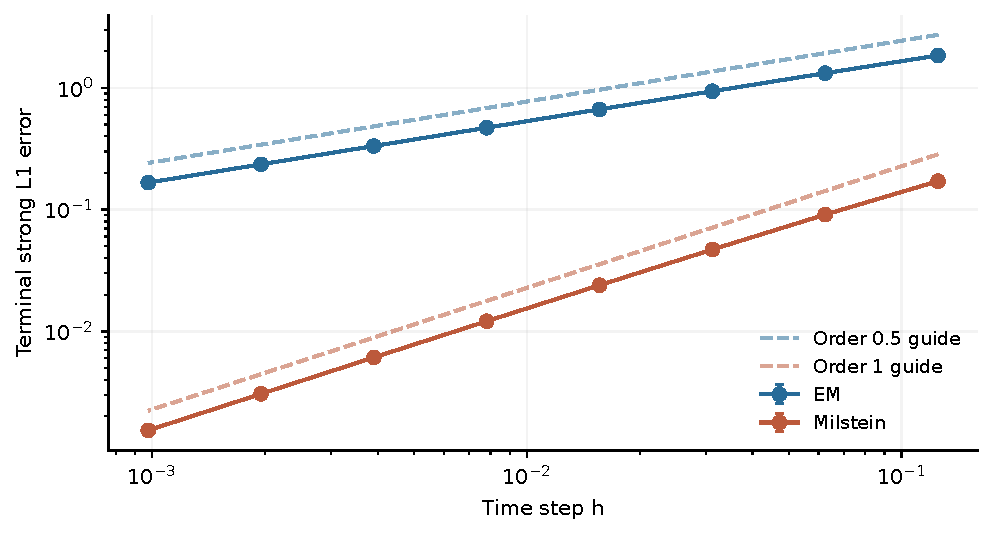
\includegraphics[width=.92\textwidth]{figures/report_gbm_strong.pdf}
\caption{Coupled GBM terminal $L^1$ error. Error bars are pointwise 95\% Monte Carlo intervals; many are smaller than the marker. Reference lines indicate orders $1/2$ and $1$.}
\end{figure}
\input{results/gbm_strong_table.tex}
The fitted slopes are \GBMEMRate{} for EM and \GBMMilRate{} for Milstein on \GBMFitWindow{}. The observed rates match the theoretical distinction: EM omits the quadratic stochastic increment, whereas Milstein accounts for it. At the finest step, Milstein has a substantially lower pathwise error. This comparison uses exactly the same Brownian paths, so differences between methods arise from the update rules rather than from different realizations of the driving noise.

The exact solution has no time-discretisation error at the simulated grid points. Small floating-point changes can occur when sums are regrouped, but these are not a convergence rate. The reported strong errors compare terminal prices rather than the maximum error over the whole path; an experiment using a path-supremum norm would be a different diagnostic.

\newpage
\subsection{Weak convergence and variance reduction}\label{sec:gbmweak}
\begin{figure}[H]\centering
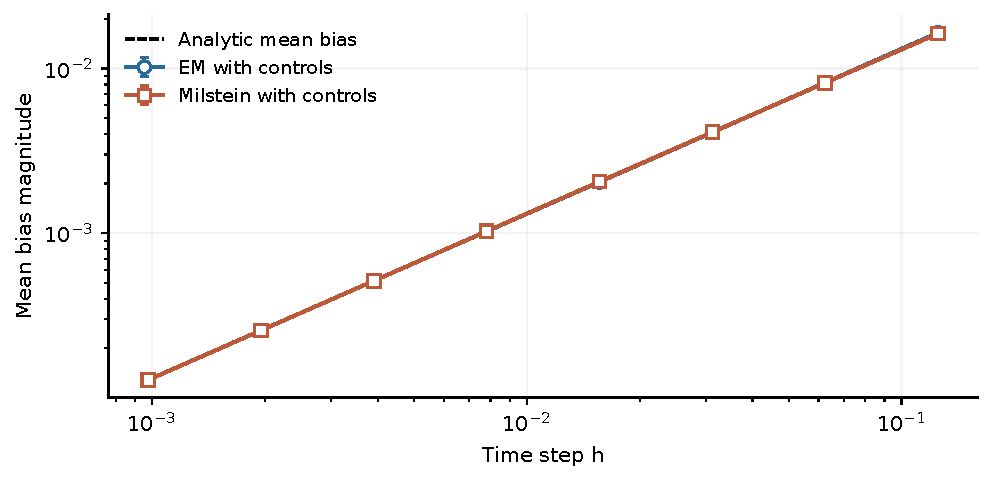
\includegraphics[width=.92\textwidth]{figures/report_gbm_weak.pdf}
\caption{GBM mean bias magnitude. Controlled paired estimates are compared with the analytic discrete-mean bias. Raw estimates and intervals remain available in the numerical tables.}
\end{figure}
\begin{table}[H]\centering\small
\caption{Signed weak bias; controlled estimates plus 95\% half-widths.}
\begin{tabular}{rrrr}\toprule
$h$ & Analytic bias & EM controlled & Milstein controlled\\\midrule
1/8 & $-1.636\times10^{-2}$ & $-1.649\times10^{-2}$ $\pm$ $1.940\times10^{-4}$ & $-1.629\times10^{-2}$ $\pm$ $9.901\times10^{-5}$\\
1/32 & $-4.102\times10^{-3}$ & $-4.096\times10^{-3}$ $\pm$ $2.811\times10^{-5}$ & $-4.106\times10^{-3}$ $\pm$ $1.399\times10^{-5}$\\
1/128 & $-1.026\times10^{-3}$ & $-1.025\times10^{-3}$ $\pm$ $3.653\times10^{-6}$ & $-1.027\times10^{-3}$ $\pm$ $1.810\times10^{-6}$\\
1/512 & $-2.566\times10^{-4}$ & $-2.567\times10^{-4}$ $\pm$ $4.660\times10^{-7}$ & $-2.566\times10^{-4}$ $\pm$ $2.301\times10^{-7}$\\
1/1024 & $-1.283\times10^{-4}$ & $-1.284\times10^{-4}$ $\pm$ $1.649\times10^{-7}$ & $-1.283\times10^{-4}$ $\pm$ $8.144\times10^{-8}$\\
\bottomrule\end{tabular}
\end{table}

The analytic bias is identical for EM and Milstein even though their strong errors differ. Its fitted order is \GBMAnalyticWeakRate{}. The controlled Monte Carlo slopes are \GBMEMWeakRate{} and \GBMMilWeakRate{} on the stated data, interpreted alongside the intervals rather than as a substitute for equation~\eqref{eq:weak}. At small $h$, an uncontrolled sample mean has far too much uncertainty to identify a bias of this size.

For completeness, let $W=\sum_n\Delta W_n$, $Q=\sum_n[(\Delta W_n)^2-h]$,
$R=\sum_n[(\Delta W_n)^3-3h\Delta W_n]$, and
$L=\exp(\sigma W-\sigma^2T/2)$. The control vector is
\begin{equation}
\begin{split}
C_1&=L-1,\quad C_2=L(W-\sigma T)/\sqrt T,\\
C_3&=L(Q-\sigma^2Th)/\sqrt{2Th},\quad
C_4=L(R-\sigma^3Th^2)/\sqrt{6Th^2},\\
C_5&=\frac{L[Q^2-(2Th+4\sigma^2Th^2+\sigma^4T^2h^2)]}{\sqrt8\,Th}.
\end{split}
\end{equation}
Gaussian exponential tilting shifts each increment's mean to $\sigma h$ while preserving variance $h$, giving $\mathbb E[C]=0$ componentwise. Production coefficients are fixed from the independent pilot. Therefore the interval describes residual sampling uncertainty without imposing the analytic bias on the estimate.

\newpage
\subsection{Distribution and positivity}
\begin{figure}[H]\centering
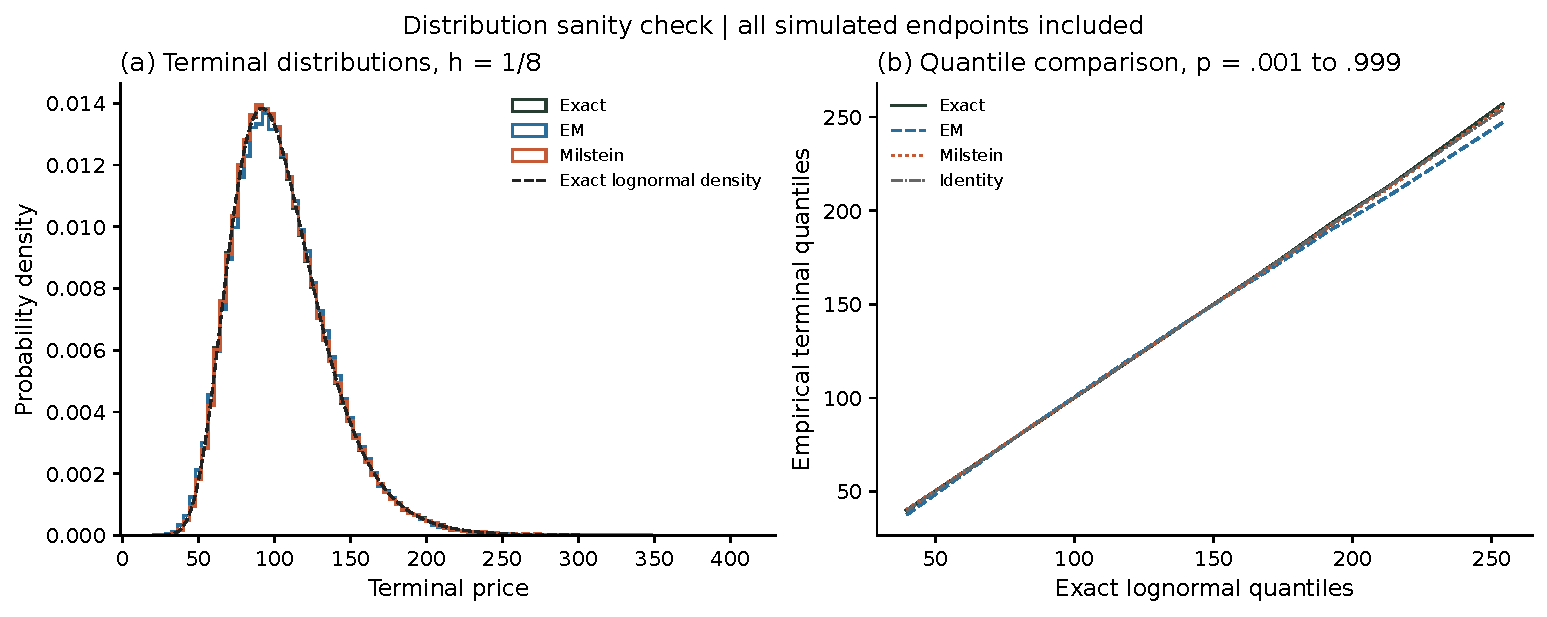
\includegraphics[width=.94\textwidth]{figures/gbm_distribution.pdf}
\caption{GBM terminal distribution compared with the exact lognormal law. The histogram is a sampling diagnostic; quantiles give a more precise distributional comparison.}
\end{figure}
\begin{table}[H]\centering\small
\caption{Terminal quantiles; numerical columns use $h=1/8$.}
\begin{tabular}{rrrrr}\toprule
$p$ & Lognormal & Exact simulation & EM & Milstein\\\midrule
0.01 & 50.012 & 49.928 & 48.387 & 50.213\\
0.05 & 61.357 & 61.378 & 60.512 & 61.615\\
0.25 & 82.091 & 82.151 & 82.303 & 82.263\\
0.50 & 100.501 & 100.557 & 101.088 & 100.582\\
0.75 & 123.041 & 123.164 & 123.653 & 123.057\\
0.95 & 164.618 & 164.485 & 163.370 & 164.043\\
0.99 & 201.961 & 202.402 & 198.376 & 201.539\\
\bottomrule\end{tabular}
\end{table}

The exact-simulation mean is \GBMExactMean{} and its variance is \GBMExactVariance{}; the mean interval is \GBMExactMeanCI{}. The analytic mean is 105.1271 and variance is 1040.7868. Sampling fluctuations in empirical moments and quantiles remain even for exact simulation; they must not be described as discretisation error.

For $S_n>0$, EM becomes negative with one-step probability
\begin{equation}
\mathbb P(S_{n+1}^{E}<0\mid S_n>0)
=\Phi\!\left(-\frac{1+\mu h}{\sigma\sqrt h}\right).
\end{equation}
For Milstein, completing the square gives the multiplier
\begin{equation}
\tfrac12\sigma^2(\Delta W+1/\sigma)^2+
\tfrac12+(\mu-\tfrac12\sigma^2)h.
\end{equation}
It can be negative only if $(\sigma^2-2\mu)h>1$. In this baseline $\sigma^2-2\mu=-0.01$, so Milstein is strictly positive for every $h>0$. In general parameter regimes this is not guaranteed. No negative prices in a finite simulation proves only what was observed; it does not make EM positivity preserving. Clipping negative values would change the method and potentially bias nonlinear payoff estimates. Neither scheme is clipped here.

\newpage
\section{Non-affine numerical results}
\subsection{Strong differences against a numerical reference}
\begin{figure}[H]\centering
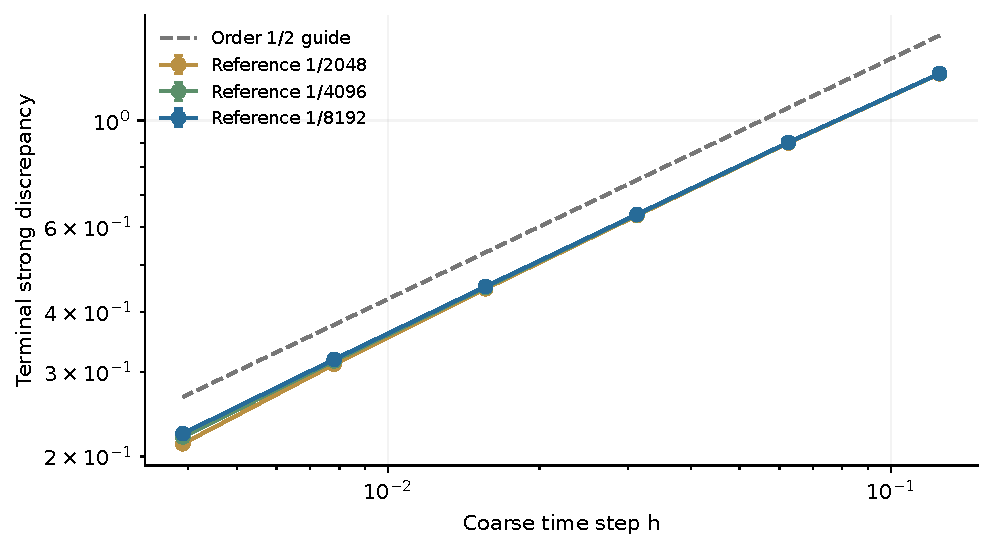
\includegraphics[width=.92\textwidth]{figures/report_nonaffine_strong.pdf}
\caption{Terminal strong differences against three coupled EM reference grids. The reference is numerical, so these are not exact-error curves.}
\end{figure}
\begin{table}[H]\centering\small
\caption{Strong discrepancy against $h_{\rm ref}=1/8192$; 95\% half-widths.}
\begin{tabular}{rrr}\toprule
$h$ & $\mathbb E|S_h-S_{\rm ref}|$ & Last reference difference / error\\\midrule
1/8 & $1.25354\pm0.00702$ & 3.2\%\\
1/16 & $0.90087\pm0.00489$ & 4.5\%\\
1/32 & $0.63818\pm0.00341$ & 6.3\%\\
1/64 & $0.45176\pm0.00241$ & 8.9\%\\
1/128 & $0.31854\pm0.00170$ & 12.6\%\\
1/256 & $0.22323\pm0.00119$ & 18.0\%\\
\bottomrule\end{tabular}
\end{table}

Against the finest reference, the empirical slope is \NARate{} over \NAFitWindow{}. The result is consistent with approximately half-order strong behavior on this window. Curves bend when a coarse grid approaches a reference grid: two nearly identical discretisations can agree well while both retain a nonzero error relative to the continuous SDE.

If $S^\star$ denotes the unknown exact terminal value, the reverse triangle inequality yields
\begin{equation}
\left|\mathbb E|S_h-S^\star|-\mathbb E|S_h-S_r|\right|
\leq \mathbb E|S_r-S^\star|.
\end{equation}
The right-hand side is unknown. Replacing $r$ by a finer grid measures sensitivity of the benchmark, not that unknown error itself. The next sections therefore report reference changes separately and avoid presenting a rate fitted through the finest coarse points as exact verification.

\newpage
\subsection{Weak payoff differences}
\begin{figure}[H]\centering
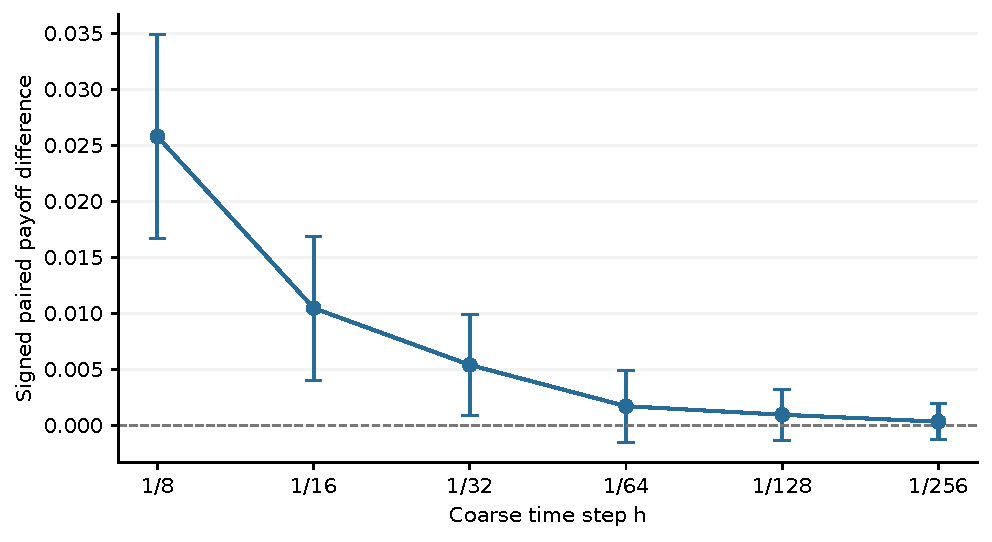
\includegraphics[width=.92\textwidth]{figures/report_nonaffine_weak.pdf}
\caption{Signed paired differences in the expected call payoff relative to the finest EM reference. Error bars are 95\% sampling intervals; the zero line identifies unresolved bias signs.}
\end{figure}
\begin{table}[H]\centering\small
\caption{Signed paired payoff differences against $h_{\rm ref}=1/8192$.}
\begin{tabular}{rrrr}\toprule
$h$ & Estimated bias & 95\% interval & Zero excluded\\\midrule
1/8 & 0.02579 & [0.01672, 0.03486] & Yes\\
1/16 & 0.01048 & [0.00405, 0.01691] & Yes\\
1/32 & 0.00540 & [0.00089, 0.00991] & Yes\\
1/64 & 0.00172 & [-0.00148, 0.00492] & No\\
1/128 & 0.00096 & [-0.00130, 0.00322] & No\\
1/256 & 0.00034 & [-0.00124, 0.00192] & No\\
\bottomrule\end{tabular}
\end{table}

\NAWeakInterpretation{}
The positive-part payoff is nonsmooth at the strike, and a weak order should not be assumed from smooth-test-function theory without further justification. The purpose of the intervals is to distinguish a visible discretisation effect from Monte Carlo noise. Common random numbers substantially reduce the variance of payoff \emph{differences}; they do not eliminate it and do not remove the numerical reference bias.

A separate first-moment check has an exact target. It\^o's lemma gives $dS=\mu S\,dt+g(Y)S\,dW^{(1)}$. Since $g$ is bounded, the associated stochastic exponential is a true martingale on the finite horizon, and $\mathbb E[S_T]=100e^{0.05}$. The log-EM scheme also satisfies
\begin{equation}
\mathbb E[S_{n+1}\mid\mathcal F_{t_n}]=e^{\mu h}S_n,
\end{equation}
because $g(Y_n)$ is known before the independent Gaussian increment. Thus its first moment is exact for any uniform step, even when its payoff expectation and individual paths are inaccurate. Agreement of the mean alone cannot establish weak accuracy for the call payoff.

\newpage
\section{Reference refinement and validation}
\begin{table}[H]\centering\small
\caption{Coupled refinement of the numerical reference.}
\begin{tabular}{rrr}\toprule
Refinement $N_a\to N_b$ & Strong difference & Signed payoff difference and 95\% CI\\\midrule
2048 $\to$ 4096 & $0.05679\pm0.00030$ & -0.000023 [-0.000423, 0.000377]\\
4096 $\to$ 8192 & $0.04016\pm0.00021$ & 0.000094 [-0.000188, 0.000376]\\
\bottomrule\end{tabular}
\end{table}

\NAReferenceInterpretation{}
\begin{table}[H]\centering
\caption{Brownian and state diagnostics at the finest non-affine grid.}
\begin{tabular}{lrr}\toprule Quantity & Observed & Target or scope\\\midrule
Increment variance 1 & $1.221\times10^{-4}$ & $1.221\times10^{-4}$\\
Increment variance 2 & $1.221\times10^{-4}$ & $1.221\times10^{-4}$\\
Increment correlation & -0.699675 & $-0.700000$\\
Sampled increments & 4,194,304 & Predetermined first batch\\
Total path updates & 1,484,000,000 & All grids\\
Finite intermediate states & Pass & $X$ and $Y$\\
Positive finite prices & Pass & All observed states\\
\bottomrule\end{tabular}

\end{table}
The variance targets for both Brownian increments are $h$, and their target correlation is $-0.7$. The diagnostics are calculated from the generated fine increments, not inferred from the generator formula. State checks include intermediate steps, because a finite terminal value alone would not rule out an invalid intermediate update.

The finest-grid mean is \NAExactMean{} with 95\% interval \NAExactMeanCI{}.
The corresponding undiscounted payoff estimate is \NAPayoff{} with interval \NAPayoffCI{}. This latter interval describes sampling uncertainty about the \emph{finest discrete model}; the refinement table is still needed to assess its bias.

This system also explains the limits of scalar Milstein. For independent Brownian drivers write $a(y)=\xi\sqrt{1+y^2}$, $c=\sqrt{1-\rho^2}$, and the diffusion columns
\begin{equation}
b_1=(g,\rho a)^\top,\qquad b_2=(0,ca)^\top .
\end{equation}
Their commutator is
\begin{equation}
(Db_2)b_1-(Db_1)b_2=(-ca\,g'(y),0)^\top\ne0.
\end{equation}
The noises are noncommutative. A general order-one multidimensional Milstein implementation needs cross terms and iterated stochastic integrals; copying the scalar GBM correction would not justify an order-one claim \cite{higham,kloeden}.

\newpage
\section{Discussion and conclusion}
The GBM experiments establish three distinct facts. First, coupling against its exact solution recovers the expected strong-order advantage of Milstein. Second, strong order and weak order answer different questions: both methods have the same first-order bias in the terminal mean despite different pathwise errors. Third, distributional and positivity checks add information that a single mean does not contain. Log-price simulation is preferable when exact GBM transitions are available, while price-based discretisation remains a useful controlled validation exercise.

For the non-affine model, bounded positive volatility and the exponential price representation give finite, positive simulated prices on the tested paths. Nested-grid comparisons provide evidence of refinement convergence and expose how a numerical benchmark can affect the measured rate. They do not produce exact errors. In particular, payoff intervals that overlap zero cannot support an asserted weak slope, and a reference residual comparable with a coarse-grid difference limits the precision of that comparison.

The main computational trade-off is between path count and temporal resolution. Halving $h$ approximately doubles updates per path. Increasing $M$ by a factor of four approximately halves the Monte Carlo standard error. Coupled differences and control variates address the sampling component, while refinement addresses discretisation. Extra paths cannot repair an underresolved reference, and smaller steps cannot by themselves remove sampling uncertainty.

The work fully addresses the SDE-specific route of Problem~4: exact--EM--Milstein comparison, strong and weak convergence with coupled paths, lognormal validation, sampling intervals, and non-affine nested-reference checks. No deterministic stability plot or scalar Milstein extension is substituted for these requirements. The numerical conclusions are limited to the stated parameter sets, horizon, error norm, sample sizes, and fitting windows.

\subsection*{Reproducibility and assistance}
The accompanying Python files generate all numerical results from fixed seeds; report tables are built directly from the saved results. Timings describe this machine and run, not portable performance guarantees. The appendix records the core updates and reproduction commands. OpenAI Codex assisted with derivations, implementation, numerical execution, and report preparation. This acknowledgement does not assert that a student has independently reviewed or approved the work.

\begin{thebibliography}{9}
\bibitem{pack} \emph{Problem Pack: Five Suggested Directions for the ODE IVP Project}.
Supplied coursework document, Direction~4, pp.~6--7.
\bibitem{higham} D.~J. Higham. An algorithmic introduction to numerical simulation of stochastic differential equations. \emph{SIAM Review}, 43(3):525--546, 2001.
\href{https://doi.org/10.1137/S0036144500378302}{doi:10.1137/S0036144500378302}.
\bibitem{kloeden} P.~E. Kloeden and E.~Platen. \emph{Numerical Solution of Stochastic Differential Equations}. Springer, 1992.
\href{https://doi.org/10.1007/978-3-662-12616-5}{doi:10.1007/978-3-662-12616-5}.
\end{thebibliography}

\newpage
\appendix
\section{Python implementation and reproduction}
The following listing states the core mathematical operations. The executable
modules additionally implement batching, control-variate pilot fitting, uncertainty estimates, diagnostics, exports, and plots; their complete source is supplied alongside this report.
\begin{lstlisting}[caption={Core SDE updates and coupled error statistics.}]
import numpy as np

def coarsen(dw_fine, n_coarse):
    m, n_fine = dw_fine.shape
    assert n_fine % n_coarse == 0
    return dw_fine.reshape(m, n_coarse, -1).sum(axis=2)

def gbm_terminal(dw, s0=100., mu=.05, sigma=.3, T=1.):
    h = T / dw.shape[1]
    exact = s0 * np.exp((mu-.5*sigma**2)*T
                         + sigma*dw.sum(axis=1))
    em = s0 * np.prod(1 + mu*h + sigma*dw, axis=1)
    mil = s0 * np.prod(1 + mu*h + sigma*dw
              + .5*sigma**2*(dw*dw-h), axis=1)
    return exact, em, mil

def log_em_step(x, y, dw1, dw2, h):
    # Values on both right-hand sides are at the old time.
    sigmoid = np.exp(-np.logaddexp(0., -y))
    g = .1 + .4*sigmoid
    x_new = x + (.05-.5*g*g)*h + g*dw1
    y_new = y + 2*(-.2-y)*h + .6*np.hypot(1.,y)*dw2
    return x_new, y_new

def mean_ci(values):
    m = len(values)
    mean = np.mean(values)
    half_width = 1.96*np.std(values, ddof=1)/np.sqrt(m)
    return mean, mean-half_width, mean+half_width

# Brownian drivers from independent standard normals:
# dw1 = sqrt(h)*z1
# dw2 = sqrt(h)*(rho*z1 + sqrt(1-rho**2)*z2)
# Strong: mean_ci(abs(s_coarse-s_reference))
# Weak: mean_ci(maximum(s_coarse-100,0)
#               -maximum(s_reference-100,0))
\end{lstlisting}
\noindent Run from the package directory using Python~3.12:
\begin{lstlisting}[numbers=none]
python -m pip install -r requirements.txt
python run_all.py
pdflatex Problem4_FinancialSDE_Coursework.tex
pdflatex Problem4_FinancialSDE_Coursework.tex
# To validate supplied results without resimulation:
python verify.py
\end{lstlisting}
\noindent\small \texttt{results/} contains machine-readable tables and logs;
\texttt{figures/} contains vector PDFs and PNGs. The supplied PDF is already compiled. The appendix listing is explanatory; the tests exercise the actual imported implementation functions. Full reproduction includes both simulation modules, while rebuilding only the report tables does not resimulate paths.
\end{document}

